\documentclass[12pt,letterpaper]{article}
\usepackage[utf8]{inputenc}
\usepackage{amsmath}
\usepackage{amsfonts}
\usepackage{amssymb}
\usepackage{graphicx}
\usepackage[left=2cm,right=2cm,top=2cm,bottom=2cm]{geometry}

\usepackage{subfigure}

\author{Tanmoy Sanyal}
\title{CMPSC 240A HW-2 Report}

\begin{document}
\maketitle

\section*{Brief code summary}
\noindent I have worked only on the model problem for this assignment. The cgsolve iterations are built into main.c and the other relevant routines \texttt{daxpy()}, \texttt{ddot()} and \texttt{matvec()} are written separately. \texttt{genB} gives a preliminary wrapper for building the vector \textbf{b} from the harness function \texttt{cs240\_getB()}. Other modifications include: changing \texttt{save\_vec()} to output input parameters and output statistics in the header of \texttt{xApprox.txt}, and an option to verify the solution using the harness function \texttt{cs240\_verify()}. Note that this option requires assembling the global vector on the root processor and is hence turned off during the scaling experiments (set up by \texttt{scaling.py}).

\noindent The communication volume for 1 \texttt{matvec()} can be calculated as:
\begin{align*}
v & = 2(p-2) * BLOCK\_SIZE + 2 * BLOCK\_SIZE \\
  & = 2(p-1)*BLOCK\_SIZE
\end{align*}
\noindent where, $BLOCK\_SIZE = n/p$ is the size of the vector passed to each processor. (A send and its corresponding receive is assumed as a single operation).

\section*{Solution verification}
\noindent The harness routine verifies my solution as correct only for small k values. Here is a graphical comparison (both cases calculated from my laptop).
%
\begin{figure*}[h]
\centering
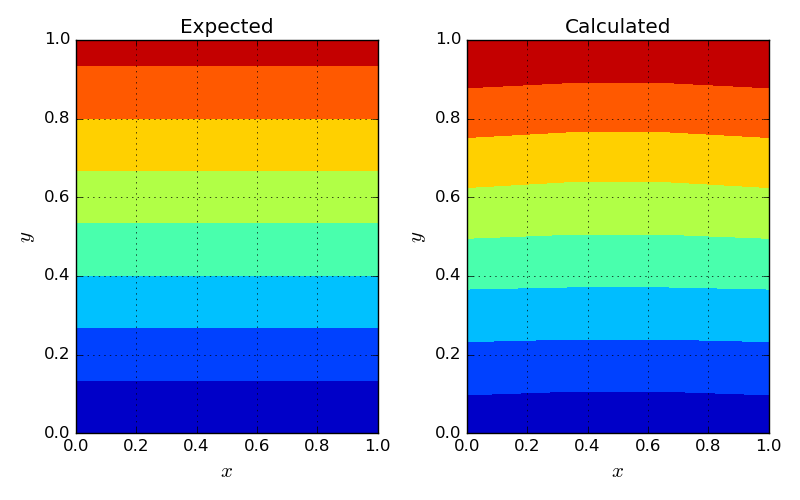
\includegraphics[scale = 0.45]{verify_k4.png}
\caption{$k = 4, p = 4, \mathrm{ maxiters} = 1000$}
\end{figure*}
%
\begin{figure*}
\centering
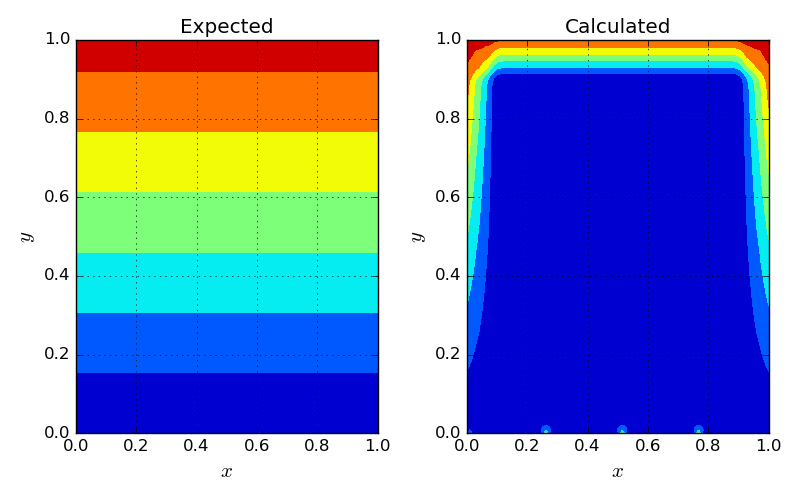
\includegraphics[scale = 0.45]{verify_k100.png}
\caption{$k = 100, p = 4, \mathrm{maxiters} = 1000$}
\end{figure*}

\section*{Scaling analyses}
\noindent The strong scaling experiment was run with $p = 1, 2, 4, 8, 12, 16, 24, 48, 72$ cores. Comet's compute nodes have cores that are multiples of 24, which guided the choice of higher $p$ values. $k = 144$ on a single processor with 1000 CG iterations was found to take around 0.26 sec. With this value of k, the strong scaling looks like:
%
\begin{figure*}[h]
\centering
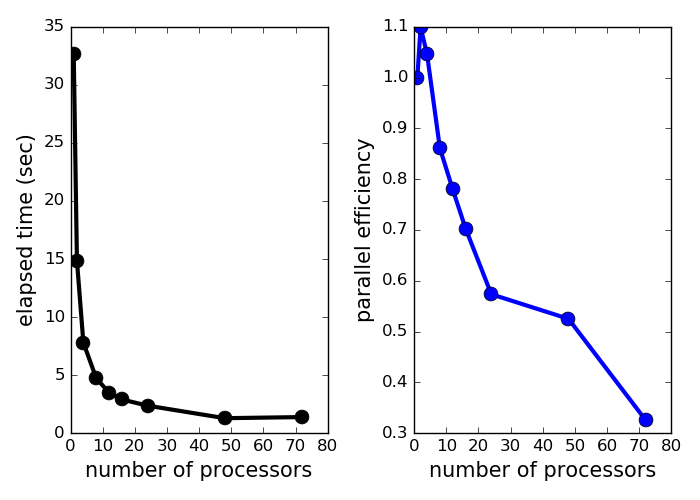
\includegraphics[scale = 0.7]{strongscale.png}
\caption{Strong scaling for $ k = 144$}
\end{figure*}

\noindent While the time taken for $p = 1$ is much lesser than the prescribed 30 sec - 1 min, this small value of $k$ helps us diagnose an important aspect from the strong scaling plot. $k = 144$ is a relatively small sized problem when distributed across many processors and so for $p \geq 24$, when the cores get distributed across nodes, the speedup is affected because of latency overhead in interprocessor communication. For a sufficiently large size problem, this change would be less noticeable.
\newpage
\noindent The weak scaling experiment used a similar number of processors as the previous case. However the first $k$ value was set at 144. Subsequent value of $k$ were chosen as $144 * \mathrm{int}(\sqrt{k})$. This ensures that $k^2/p$ is always an integer and the tests run fast, even with 1000 iterations of the CG loop. The weak scaling is:
%
\begin{figure*}[h]
\centering
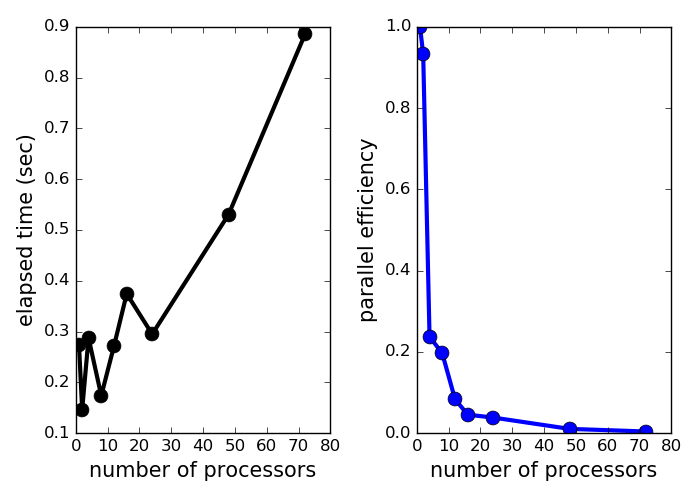
\includegraphics[scale = 0.7]{weakscale.png}
\caption{Weak scaling for $ k = 144, 144, 288, 288, 432, 576, 576, 864, 1152$}
\end{figure*}

\noindent In weak scaling, the problem size grows with the number of processors, which is primarily responsible for sublinear speedup. However, this also means that the problem size on each processor is tailored to be comparable to the corresponding memory requirement, which further tips the effective latency - computation balance. So latency overhead effects start appearing not across nodes but also across cores within the same node.

\section*{Profiling with tau and pprof}
\noindent I ran the profiling experiment (using tau and pprof) with $k = 100$ and 10 CG iterations for processor numbers similar to the one in the scaling experiment. Since, $k^2/p$ is an integer by design, this code is ``embarassingly" parallel. Also, it is simple to calculate the total number of calls for each function by hand (following an approach similar to calculating the communication volume). So, I will report only the total inclusive times for the different routines and analyze their trends with increasing number of processors.
\\
\begin{figure*}[h]
\flushleft
\includegraphics[scale = 0.3]{tauprof.png}
\caption{Runtimes of different routines (profiled with tau)}
\end{figure*}

\noindent \texttt{daxpy} and \texttt{gen\_B} are essentially serial routines without any message passing; their run times are only dependent on their corresponding works and so speedup is approximately linear. \texttt{gen\_B} slows down a little, since it involves extracting the processor rank (using \texttt{MPI\_COMM\_RANK}). On the other hand, the \texttt{Send} and \texttt{Recv} routines become slower with increasing number of processors and are hit severely when processors span different nodes. This performance hit is also apparent in \texttt{MPI\_Allreduce} and \texttt{ddot} (which uses \texttt{Allreduce} and so has an exactly similar trend).

\noindent The conflict between decreasing per-processor work and increasing communication overhead, plays out in \texttt{matvec} which is efficient while going from 1 to 2 or 4 processors, but then doesn't become any faster and in fact takes more time when multiple nodes are used.\\ 

\noindent It may be possible to fit all of these plots individually to a latency-bandwith model and estimate parameters separately, which can be then suitably combined to produce very accurate latency estimates for Comet compute nodes.

\end{document}